\chapter{Signs}
	\section{Introduction}
	\paragraph{}Signs main objective is to give some information to the pilots about what lies ahead in order to guarantee the perfect organisation and efficiency of the aircraft trajectory while on taxiways. 
	
	The criteria used in order to dimension and calculate the position of each sign can be obtained from a table stated on the point 5.4 of the Annex 14.
	
	\begin{figure}[H]
		\centering
		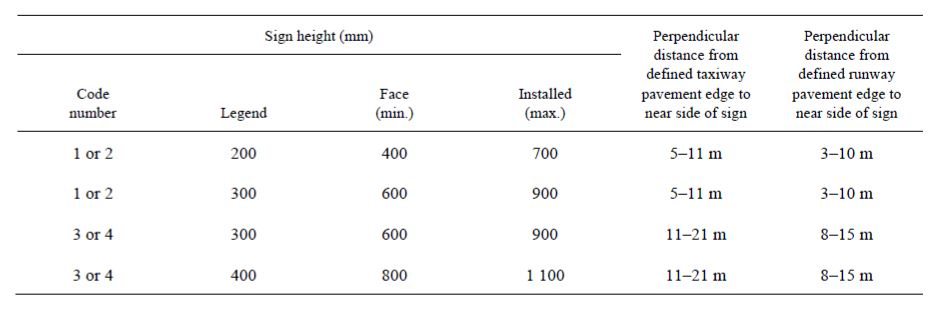
\includegraphics[clip, trim=0cm 0cm 0cm 0cm, width=0.95\textwidth]{./images/Annex14/signstable}
		\caption{Location distances for taxiing guidance signs.} %nom de la figura
		\label{} %per denotar una referencia
	\end{figure}

	Since the airport designed has a number reference of 4, the distance from the runway to the sign will be 12m and the distance from the taxiways will be 15m. Two different values have been chosen in order to help the pilots differentiate which sign are they looking at. 
	
	Another important aspect to be taken into account is the fact that all the signs will have inside illumination in order to allow the night time operations.
	
	\section{Mandatory instruction signs}
	\textbf{\textit{Application}}
	
	A mandatory instruction sign shall be provided to identify a location beyond which an aircraft taxiing or vehicle shall not proceed unless authorized by the aerodrome control tower. The signs included in this section are: designation signs, category I, II or III holding position signs, runway-holding position signs, road-holding position signs and NO ENTRY signs.
	
	\textbf{\textit{Location}}
	
	The location of each sign depend on the prohibition or the information they are giving:
	
	- A runway designation sign at a taxiway/runway intersection or a runway/runway intersection shall be located on each side of the runway-holding position marking facing the direction of approach to the runway.
	
	- A category I, II or III holding position sign shall be located on each side of the runway-holding position marking facing the direction of the approach to the critical area.
	
	- A NO ENTRY sign shall be located at the beginning of the area to which entrance is prohibited on each side of the taxiway as viewed by the pilot.
	
	\textbf{\textit{Characteristics}}
	
	A mandatory instruction sign shall consist of an inscription in white on a red background. Furthermore, in the specific case of inscription on a category I, II, III, joint II/III or joint I/II/III holding position sign shall consist of the runway designator, it must be followed by CAT I, CAT II, CAT III, CAT II/III or CAT I/II/III, as appropriate.
	
	\textbf{\textit{Examples}}
	
	Now that the mandatory instruction signs have been fully explained and defined, the next step is to place those signs in the airport. Some examples of the sign placed will be shown and explained:
	
	The NO ENTRY sing have been installed at the beginning of every rapid exit taxiway in both sides in order to aware the pilot that those taxiways are only allowed for the planes that land to exit the runway, entering the runway through a rapid exit way is strictly forbidden. The next figure shows the sign mentioned above:
	
	\begin{figure}[H]
		\centering
		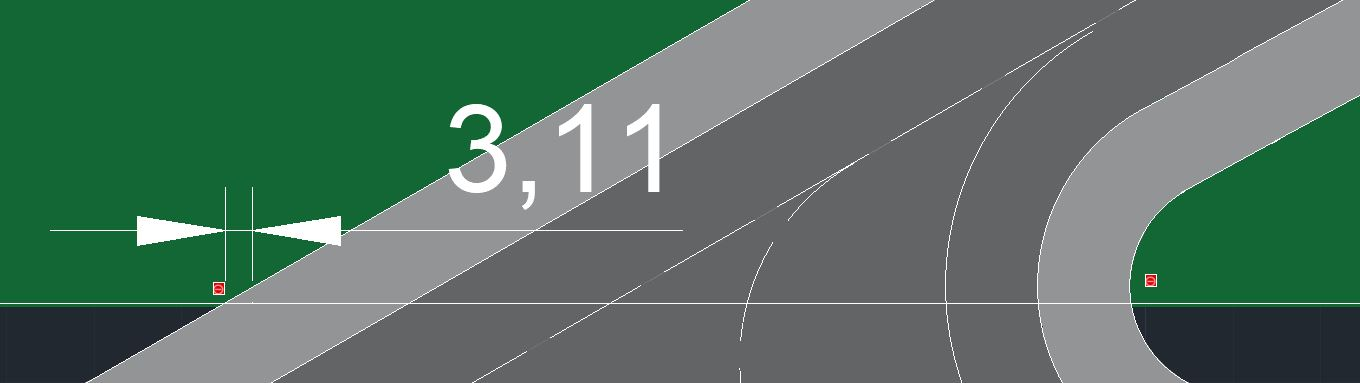
\includegraphics[clip, trim=0cm 0cm 0cm 0cm, width=0.95\textwidth]{./images/signsexamples/NOentrysign}
		\caption{No entry sign positioning and example.} %nom de la figura
		\label{} %per denotar una referencia
	\end{figure}
	 
	The following sign is used in order to indicate the holding position and has to be placed in both sides of the runway that leads to that critical area:
	
	\begin{figure}[H]
		\centering
		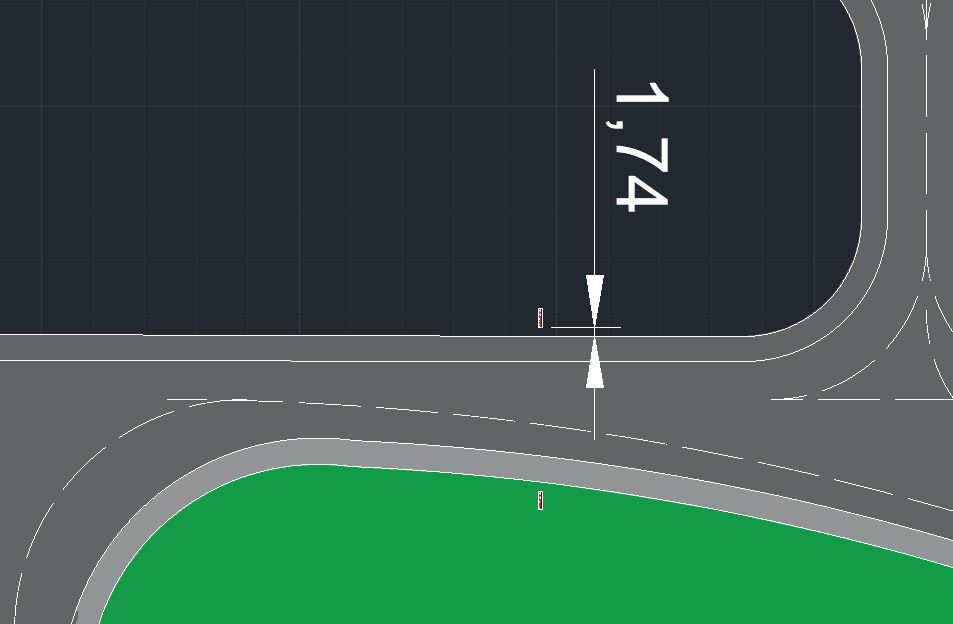
\includegraphics[clip, trim=0cm 0cm 0cm 0cm, width=0.95\textwidth]{./images/signsexamples/holdingposition}
		\caption{Holding positioning sign.} %nom de la figura
		\label{} %per denotar una referencia
	\end{figure}
	
	Since the sings can not be appreciated in the images due to the difference on the scale, some of the signs mentioned above will be shown in a bigger scale:
	
	\begin{figure}[H]
		\centering
		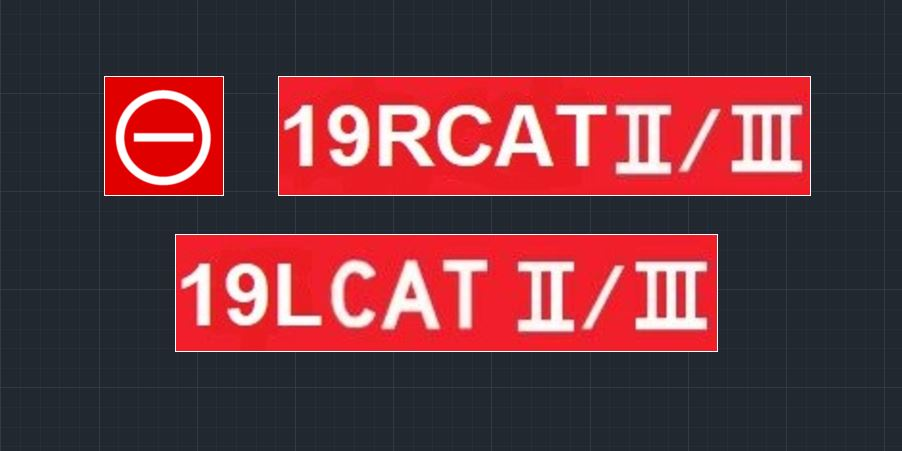
\includegraphics[clip, trim=0cm 0cm 0cm 0cm, width=0.8\textwidth]{./images/signsexamples/examples}
		\caption{Examples of the mandatory instruction signs used in the airport.} %nom de la figura
		\label{} %per denotar una referencia
	\end{figure}
	
	As it can be seen, both runways have their holding position in the direction 19, thus they have to be differentiated by an R (right) or L (Left), depending on the runway. Furthermore, the sign also displays information about the runway category. The other sign shown in the figure is the no entry sign.
	
	\section{Information signs}
	\textbf{\textit{Application}}
	
	An information sign shall be provided where there is an operational need to identify by a sign, a specific location, or routing information. Furthermore, information signs shall include: direction signs, location signs, destination signs, runway exit signs, runway vacated signs and intersection take-off signs.
	
	\textbf{\textit{Location}}
	
	Wherever practicable, the signs must be located on the left-hand side of the taxiway in accordance with table shown at the beginning of the section. Depending on the information sign, they get a different location:
	
	-At a taxiway intersection, information signs shall be located prior to the intersection and in line with the intermediate holding position marking. Where there is no intermediate holding position marking, the signs shall be installed at least 60 m from the centre line of the intersecting taxiway where the code number is 3 or 4, and at least 40 m where the code number is 1 or 2.
	
	- A runway exit sign shall be located prior to the runway exit point in line with a position at least 60 m prior to the point of tangency where the code number is 3 or 4, and at least 30 m where the code number is 1 or 2.
	
	\textbf{\textit{Characteristics}}
	
	A location sign shall consist of an inscription in yellow on a black background and where it is a stand-alone sign shall have a yellow border and the inscription on a runway exit sign shall consist of the designator of the exit taxiway and an arrow indicating the direction to follow.
	
	\textbf{\textit{Examples}}
	
	As for the mandatory instruction signs, now that the information signs have been defined, some examples will be given in order to ease the understanding of their function: 
	
	The first signs that will be exemplified will be the available runway length information signs. Those signs are placed in the entrance to the runway and give the available length that the aircraft has in order to perform the takeoff. Generally, they are only given in one side of the intersection. 
	
	\begin{figure}[H]
		\centering
		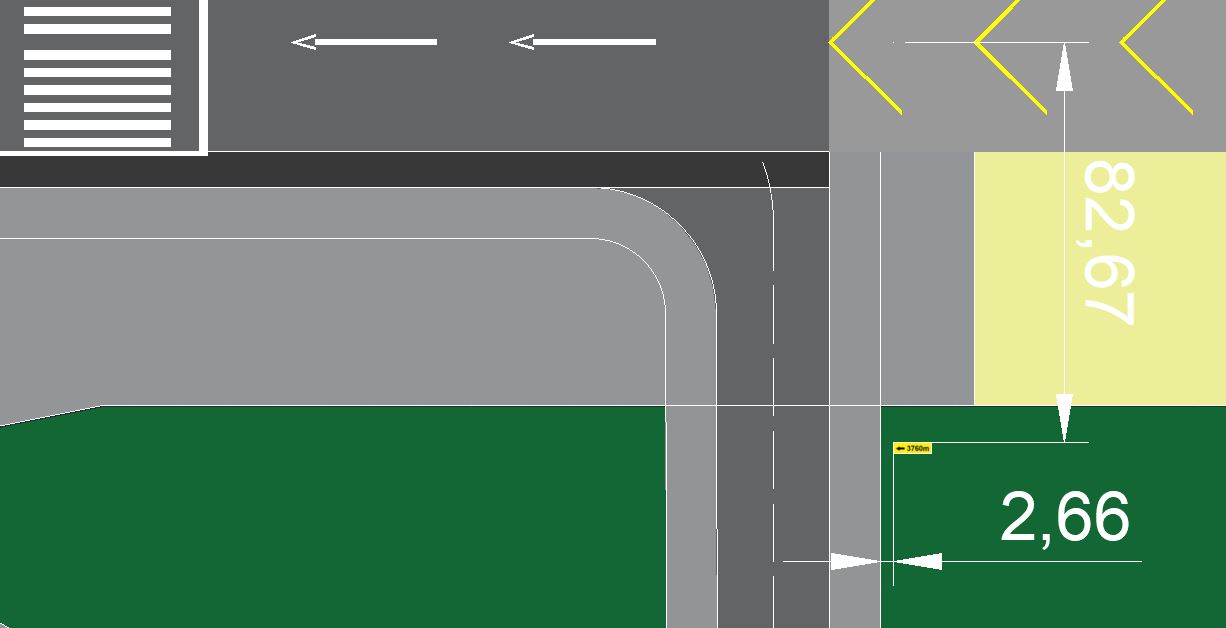
\includegraphics[clip, trim=0cm 0cm 0cm 0cm, width=0.8\textwidth]{./images/signsexamples/TODAsign}
		\caption{Available length information sign positioning.} %nom de la figura
		\label{} %per denotar una referencia
	\end{figure}

	The next signs that will also be explained are the ones that show information about the exit runway letter after landing. Each exit has assigned a different letter, thus there is one sign for each exit and rapid exit. All the signs will be place at the same distance from the runway. 
	
	\begin{figure}[H]
		\centering
		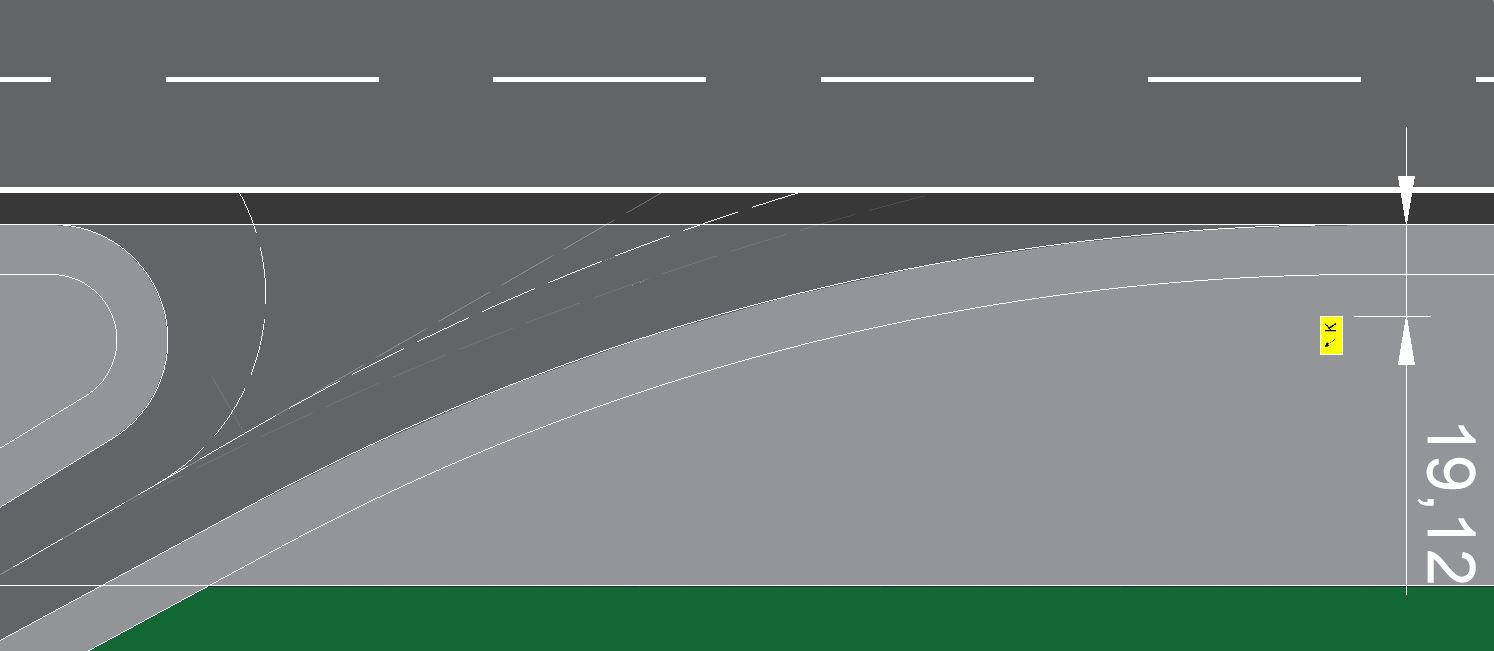
\includegraphics[clip, trim=0cm 0cm 0cm 0cm, width=0.8\textwidth]{./images/signsexamples/exitexample}
		\caption{Exit runway sign distances and positioning.} %nom de la figura
		\label{} %per denotar una referencia
	\end{figure}

	Finally, an image with some of the informative sign will be shown:
	
	\begin{figure}[H]
		\centering
		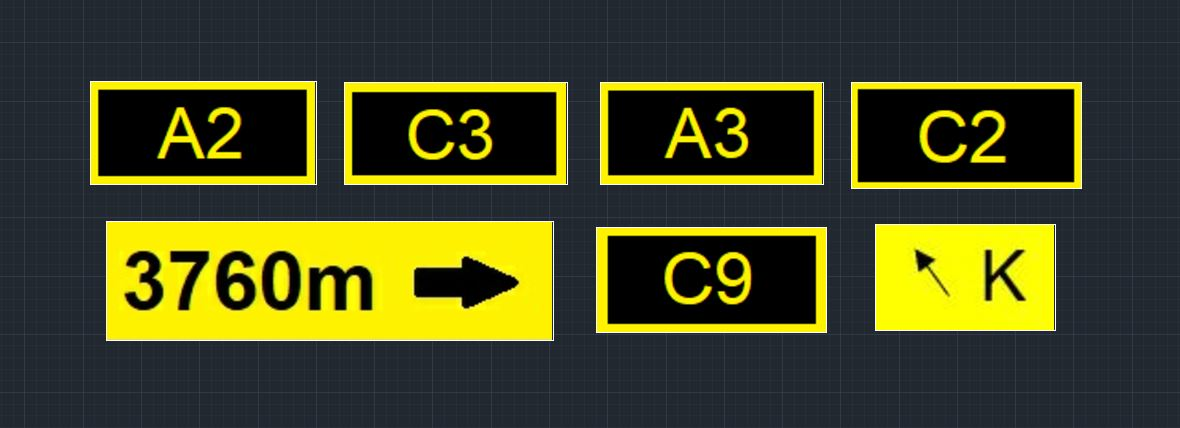
\includegraphics[clip, trim=0cm 0cm 0cm 0cm, width=0.8\textwidth]{./images/signsexamples/exempleinf}
		\caption{Exit runway sign distances and positioning.} %nom de la figura
		\label{} %per denotar una referencia
	\end{figure}
	
	The signs with black background and a yellow rectangle are the signs used in order to inform the pilot which is his current location. 
	

	